\documentclass[twoside]{book}

% Packages required by doxygen
\usepackage{fixltx2e}
\usepackage{calc}
\usepackage{doxygen}
\usepackage[export]{adjustbox} % also loads graphicx
\usepackage{graphicx}
\usepackage[utf8]{inputenc}
\usepackage{makeidx}
\usepackage{multicol}
\usepackage{multirow}
\PassOptionsToPackage{warn}{textcomp}
\usepackage{textcomp}
\usepackage[nointegrals]{wasysym}
\usepackage[table]{xcolor}

% Font selection
\usepackage[T1]{fontenc}
\usepackage[scaled=.90]{helvet}
\usepackage{courier}
\usepackage{amssymb}
\usepackage{sectsty}
\renewcommand{\familydefault}{\sfdefault}
\allsectionsfont{%
  \fontseries{bc}\selectfont%
  \color{darkgray}%
}
\renewcommand{\DoxyLabelFont}{%
  \fontseries{bc}\selectfont%
  \color{darkgray}%
}
\newcommand{\+}{\discretionary{\mbox{\scriptsize$\hookleftarrow$}}{}{}}

% Page & text layout
\usepackage{geometry}
\geometry{%
  a4paper,%
  top=2.5cm,%
  bottom=2.5cm,%
  left=2.5cm,%
  right=2.5cm%
}
\tolerance=750
\hfuzz=15pt
\hbadness=750
\setlength{\emergencystretch}{15pt}
\setlength{\parindent}{0cm}
\setlength{\parskip}{3ex plus 2ex minus 2ex}
\makeatletter
\renewcommand{\paragraph}{%
  \@startsection{paragraph}{4}{0ex}{-1.0ex}{1.0ex}{%
    \normalfont\normalsize\bfseries\SS@parafont%
  }%
}
\renewcommand{\subparagraph}{%
  \@startsection{subparagraph}{5}{0ex}{-1.0ex}{1.0ex}{%
    \normalfont\normalsize\bfseries\SS@subparafont%
  }%
}
\makeatother

% Headers & footers
\usepackage{fancyhdr}
\pagestyle{fancyplain}
\fancyhead[LE]{\fancyplain{}{\bfseries\thepage}}
\fancyhead[CE]{\fancyplain{}{}}
\fancyhead[RE]{\fancyplain{}{\bfseries\leftmark}}
\fancyhead[LO]{\fancyplain{}{\bfseries\rightmark}}
\fancyhead[CO]{\fancyplain{}{}}
\fancyhead[RO]{\fancyplain{}{\bfseries\thepage}}
\fancyfoot[LE]{\fancyplain{}{}}
\fancyfoot[CE]{\fancyplain{}{}}
\fancyfoot[RE]{\fancyplain{}{\bfseries\scriptsize Generated by Doxygen }}
\fancyfoot[LO]{\fancyplain{}{\bfseries\scriptsize Generated by Doxygen }}
\fancyfoot[CO]{\fancyplain{}{}}
\fancyfoot[RO]{\fancyplain{}{}}
\renewcommand{\footrulewidth}{0.4pt}
\renewcommand{\chaptermark}[1]{%
  \markboth{#1}{}%
}
\renewcommand{\sectionmark}[1]{%
  \markright{\thesection\ #1}%
}

% Indices & bibliography
\usepackage{natbib}
\usepackage[titles]{tocloft}
\setcounter{tocdepth}{3}
\setcounter{secnumdepth}{5}
\makeindex

% Hyperlinks (required, but should be loaded last)
\usepackage{ifpdf}
\ifpdf
  \usepackage[pdftex,pagebackref=true]{hyperref}
\else
  \usepackage[ps2pdf,pagebackref=true]{hyperref}
\fi
\hypersetup{%
  colorlinks=true,%
  linkcolor=blue,%
  citecolor=blue,%
  unicode%
}

% Custom commands
\newcommand{\clearemptydoublepage}{%
  \newpage{\pagestyle{empty}\cleardoublepage}%
}

\usepackage{caption}
\captionsetup{labelsep=space,justification=centering,font={bf},singlelinecheck=off,skip=4pt,position=top}

%===== C O N T E N T S =====

\begin{document}

% Titlepage & ToC
\hypersetup{pageanchor=false,
             bookmarksnumbered=true,
             pdfencoding=unicode
            }
\pagenumbering{roman}
\begin{titlepage}
\vspace*{7cm}
\begin{center}%
{\Large Enchain \\[1ex]\large v1.\+0.\+0 }\\
\vspace*{1cm}
{\large Generated by Doxygen 1.8.11}\\
\end{center}
\end{titlepage}
\clearemptydoublepage
\tableofcontents
\clearemptydoublepage
\pagenumbering{arabic}
\hypersetup{pageanchor=true}

%--- Begin generated contents ---
\chapter{R\+E\+A\+D\+ME}
\label{md_README}
\hypertarget{md_README}{}
\#\href{https://github.com/Zhehua-Hu/Enchain}{\tt }Enchain(under construction)

Enchain is a versatile imag$\ast$$\ast$\+E$\ast$$\ast$ labelli$\ast$$\ast$\+N$\ast$$\ast$g tool$\ast$$\ast$\+C\+H\+A\+I\+N$\ast$$\ast$ for deep learning.

It is a guidance/pipeline to prepare your own dataset.

\subsection*{Dataset Generation Procedure}

 \subsection*{Installation}


\begin{DoxyItemize}
\item Binary Execuable File
\begin{DoxyItemize}
\item \mbox{[}Windows\mbox{]}() (Tested on win7)
\item \mbox{[}Linux\mbox{]}() (Tested on Ubuntu16.\+04)
\end{DoxyItemize}
\item Compile From Source Code ``` blabla... ``` \subsection*{Usage}
\end{DoxyItemize}

\subsection*{Development Environment}


\begin{DoxyItemize}
\item Ubuntu 16.\+04.\+1 L\+TS x64
\item Open\+C\+V3.\+1
\item Python2.\+7
\item Py\+Qt5.\+8
\end{DoxyItemize}

\section*{Join us!}

\subsection*{Acknowladgement}

Icons\+:https\+://github.com/\+Templarian/\+Material\+Design

\subsection*{License}

\subsection*{Related}
\chapter{Tiny Demo First}
\label{md_TODO}
\hypertarget{md_TODO}{}
Page 1
\begin{DoxyItemize}
\item {\bfseries image\+\_\+select}
\end{DoxyItemize}

Page 2 Guandance Label\+Img

Page 3 Guandance image\+\_\+check

\section*{}
\chapter{Hierarchical Index}
\section{Class Hierarchy}
This inheritance list is sorted roughly, but not completely, alphabetically\+:\begin{DoxyCompactList}
\item \contentsline{section}{Enchain.\+Img\+List}{\pageref{classEnchain_1_1ImgList}}{}
\item Q\+Main\+Window\begin{DoxyCompactList}
\item \contentsline{section}{Enchain.\+Main\+Window}{\pageref{classEnchain_1_1MainWindow}}{}
\end{DoxyCompactList}
\item Ui\+\_\+\+Main\+Window\begin{DoxyCompactList}
\item \contentsline{section}{Enchain.\+Main\+Window}{\pageref{classEnchain_1_1MainWindow}}{}
\end{DoxyCompactList}
\end{DoxyCompactList}

\chapter{Class Index}
\section{Class List}
Here are the classes, structs, unions and interfaces with brief descriptions\+:\begin{DoxyCompactList}
\item\contentsline{section}{\hyperlink{classEnchain_1_1ImgList}{Enchain.\+Img\+List} }{\pageref{classEnchain_1_1ImgList}}{}
\item\contentsline{section}{\hyperlink{classEnchain_1_1MainWindow}{Enchain.\+Main\+Window} }{\pageref{classEnchain_1_1MainWindow}}{}
\end{DoxyCompactList}

\chapter{Class Documentation}
\hypertarget{classEnchain_1_1ImgList}{}\section{Enchain.\+Img\+List Class Reference}
\label{classEnchain_1_1ImgList}\index{Enchain.\+Img\+List@{Enchain.\+Img\+List}}
\subsection*{Public Member Functions}
\begin{DoxyCompactItemize}
\item 
def {\bfseries \+\_\+\+\_\+init\+\_\+\+\_\+} (self, folder)\hypertarget{classEnchain_1_1ImgList_ad0c2329676c49fb4f5d7c9cfb2891140}{}\label{classEnchain_1_1ImgList_ad0c2329676c49fb4f5d7c9cfb2891140}

\item 
def {\bfseries get\+Contained\+Imgs} (self, folder, type=\char`\"{}Not\+Recursive\char`\"{})\hypertarget{classEnchain_1_1ImgList_a5db106b9f9b6b5b6561061d6fd4b6ad5}{}\label{classEnchain_1_1ImgList_a5db106b9f9b6b5b6561061d6fd4b6ad5}

\item 
def {\bfseries First\+Img} (self)\hypertarget{classEnchain_1_1ImgList_af3b8190bfe73613f139d70c87dfef006}{}\label{classEnchain_1_1ImgList_af3b8190bfe73613f139d70c87dfef006}

\item 
def {\bfseries next\+Img} (self)\hypertarget{classEnchain_1_1ImgList_a5bf5c2f72a59f91838a2986be48b50ac}{}\label{classEnchain_1_1ImgList_a5bf5c2f72a59f91838a2986be48b50ac}

\item 
def {\bfseries previous\+Img} (self)\hypertarget{classEnchain_1_1ImgList_ae986be383da7305bf921f3190827996a}{}\label{classEnchain_1_1ImgList_ae986be383da7305bf921f3190827996a}

\item 
def {\bfseries safe\+Limit} (self, idx)\hypertarget{classEnchain_1_1ImgList_a0d9f0228c7a5bb3466303786e2ee5596}{}\label{classEnchain_1_1ImgList_a0d9f0228c7a5bb3466303786e2ee5596}

\item 
def {\bfseries \+\_\+\+\_\+repr\+\_\+\+\_\+} (self)\hypertarget{classEnchain_1_1ImgList_aae29610f2afed38619ed598002ffef86}{}\label{classEnchain_1_1ImgList_aae29610f2afed38619ed598002ffef86}

\end{DoxyCompactItemize}
\subsection*{Public Attributes}
\begin{DoxyCompactItemize}
\item 
{\bfseries img\+\_\+dirname}\hypertarget{classEnchain_1_1ImgList_ad465be8e484cb5d7690d3c25ef619350}{}\label{classEnchain_1_1ImgList_ad465be8e484cb5d7690d3c25ef619350}

\item 
{\bfseries img\+\_\+cnt}\hypertarget{classEnchain_1_1ImgList_ae02ad449877d9c92ecb0477c70c2c915}{}\label{classEnchain_1_1ImgList_ae02ad449877d9c92ecb0477c70c2c915}

\item 
{\bfseries cur\+\_\+idx}\hypertarget{classEnchain_1_1ImgList_a3fc42ff6a5b94e104e0d234b56a92b3f}{}\label{classEnchain_1_1ImgList_a3fc42ff6a5b94e104e0d234b56a92b3f}

\end{DoxyCompactItemize}
\subsection*{Static Public Attributes}
\begin{DoxyCompactItemize}
\item 
int {\bfseries cur\+\_\+idx} = 0\hypertarget{classEnchain_1_1ImgList_a6598597dce46ff6a28c66f0d774b66fb}{}\label{classEnchain_1_1ImgList_a6598597dce46ff6a28c66f0d774b66fb}

\item 
int {\bfseries img\+\_\+cnt} = 0\hypertarget{classEnchain_1_1ImgList_a762bd9dd47d42bf2a8d83bd4a118d8b7}{}\label{classEnchain_1_1ImgList_a762bd9dd47d42bf2a8d83bd4a118d8b7}

\end{DoxyCompactItemize}


\subsection{Detailed Description}
\begin{DoxyVerb}class: provide image list management
\end{DoxyVerb}
 

The documentation for this class was generated from the following file\+:\begin{DoxyCompactItemize}
\item 
Enchain.\+py\end{DoxyCompactItemize}

\hypertarget{classEnchain_1_1MainWindow}{}\section{Enchain.\+Main\+Window Class Reference}
\label{classEnchain_1_1MainWindow}\index{Enchain.\+Main\+Window@{Enchain.\+Main\+Window}}


Inheritance diagram for Enchain.\+Main\+Window\+:\nopagebreak
\begin{figure}[H]
\begin{center}
\leavevmode
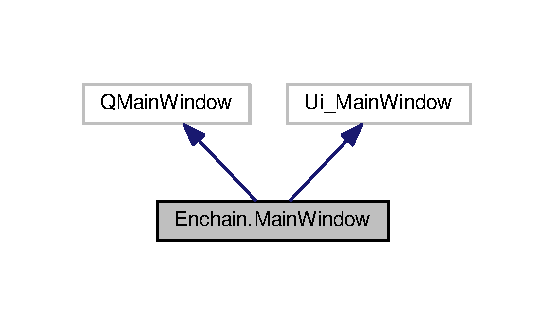
\includegraphics[width=266pt]{classEnchain_1_1MainWindow__inherit__graph}
\end{center}
\end{figure}


Collaboration diagram for Enchain.\+Main\+Window\+:\nopagebreak
\begin{figure}[H]
\begin{center}
\leavevmode
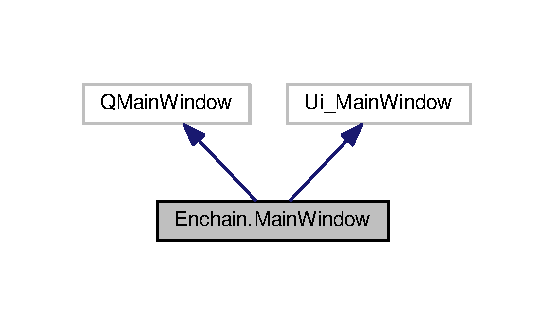
\includegraphics[width=266pt]{classEnchain_1_1MainWindow__coll__graph}
\end{center}
\end{figure}
\subsection*{Public Member Functions}
\begin{DoxyCompactItemize}
\item 
def {\bfseries \+\_\+\+\_\+init\+\_\+\+\_\+} (self, parent=None)\hypertarget{classEnchain_1_1MainWindow_a7f0e08facb3dfa0491954c7ceb5b4b58}{}\label{classEnchain_1_1MainWindow_a7f0e08facb3dfa0491954c7ceb5b4b58}

\item 
def {\bfseries setup\+Menubar} (self)\hypertarget{classEnchain_1_1MainWindow_ab61ba6fe3f0aa7f38186764edcdbbe83}{}\label{classEnchain_1_1MainWindow_ab61ba6fe3f0aa7f38186764edcdbbe83}

\item 
def {\bfseries setup\+Toolbar} (self)\hypertarget{classEnchain_1_1MainWindow_af4f255cd0632e3cb349c4df086958846}{}\label{classEnchain_1_1MainWindow_af4f255cd0632e3cb349c4df086958846}

\item 
def {\bfseries setup\+Buttons} (self)\hypertarget{classEnchain_1_1MainWindow_aaf6eb5f3f030979fcf95a874fe5dac03}{}\label{classEnchain_1_1MainWindow_aaf6eb5f3f030979fcf95a874fe5dac03}

\item 
def {\bfseries setup\+Statusbar} (self)\hypertarget{classEnchain_1_1MainWindow_a6c17e4aed6d8b32d6188fba360710419}{}\label{classEnchain_1_1MainWindow_a6c17e4aed6d8b32d6188fba360710419}

\item 
def {\bfseries print\+To\+Status} (self, message)\hypertarget{classEnchain_1_1MainWindow_ad892d70ac25c1e02b87f5cf324be0108}{}\label{classEnchain_1_1MainWindow_ad892d70ac25c1e02b87f5cf324be0108}

\item 
def {\bfseries open\+Image} (self)\hypertarget{classEnchain_1_1MainWindow_affd03c35f9e579386c3d4e27099bc17d}{}\label{classEnchain_1_1MainWindow_affd03c35f9e579386c3d4e27099bc17d}

\item 
def {\bfseries show\+Img} (self, img\+\_\+path)\hypertarget{classEnchain_1_1MainWindow_acecbe623251e65191209eae62f77693b}{}\label{classEnchain_1_1MainWindow_acecbe623251e65191209eae62f77693b}

\item 
def {\bfseries get\+Pixmap} (self, img\+\_\+path)\hypertarget{classEnchain_1_1MainWindow_a5f3f4302aa4180d5e50f246899f1aaba}{}\label{classEnchain_1_1MainWindow_a5f3f4302aa4180d5e50f246899f1aaba}

\item 
def {\bfseries update\+View} (self, qpixmap)\hypertarget{classEnchain_1_1MainWindow_a5f45d47c0a2c4d499990b218b30d1b79}{}\label{classEnchain_1_1MainWindow_a5f45d47c0a2c4d499990b218b30d1b79}

\item 
def {\bfseries clear\+View} (self)\hypertarget{classEnchain_1_1MainWindow_af8199aed66ca8aa96782ec4f84f6b085}{}\label{classEnchain_1_1MainWindow_af8199aed66ca8aa96782ec4f84f6b085}

\item 
def {\bfseries set\+Workspace} (self)\hypertarget{classEnchain_1_1MainWindow_aebc0385b704f35219927843ad2a05f44}{}\label{classEnchain_1_1MainWindow_aebc0385b704f35219927843ad2a05f44}

\item 
def {\bfseries show\+Next\+Img} (self)\hypertarget{classEnchain_1_1MainWindow_a16cea5f6dfc627ad80861f3f65d726f0}{}\label{classEnchain_1_1MainWindow_a16cea5f6dfc627ad80861f3f65d726f0}

\item 
def {\bfseries show\+Previous\+Img} (self)\hypertarget{classEnchain_1_1MainWindow_a333cbdd2c65818a4073dfe06ee205db6}{}\label{classEnchain_1_1MainWindow_a333cbdd2c65818a4073dfe06ee205db6}

\item 
def {\bfseries select\+Img} (self)\hypertarget{classEnchain_1_1MainWindow_a354c93ca25f09c29c858aad2dfebaab8}{}\label{classEnchain_1_1MainWindow_a354c93ca25f09c29c858aad2dfebaab8}

\item 
def {\bfseries convert\+\_\+\+Cv\+Img\+To\+Q\+Pixmap} (self, cv\+Image)\hypertarget{classEnchain_1_1MainWindow_a86e559ec504749fb5e432fe90c064290}{}\label{classEnchain_1_1MainWindow_a86e559ec504749fb5e432fe90c064290}

\item 
def {\bfseries convert\+\_\+\+Cv\+Img\+To\+Q\+Img} (self, cv\+Image)\hypertarget{classEnchain_1_1MainWindow_a089138200e6bf164896bf2db443f7262}{}\label{classEnchain_1_1MainWindow_a089138200e6bf164896bf2db443f7262}

\item 
def {\bfseries Save\+Image} (self)\hypertarget{classEnchain_1_1MainWindow_a3e0b16b3227213e2f2ee7429681f0ee5}{}\label{classEnchain_1_1MainWindow_a3e0b16b3227213e2f2ee7429681f0ee5}

\item 
def {\bfseries get\+Contained\+Files} (self, folder, type=\char`\"{}Not\+Recursive\char`\"{})\hypertarget{classEnchain_1_1MainWindow_a12fc7938fcf2c0f15a9cf5eb2d4a8636}{}\label{classEnchain_1_1MainWindow_a12fc7938fcf2c0f15a9cf5eb2d4a8636}

\item 
def {\bfseries close\+Event} (self, event)\hypertarget{classEnchain_1_1MainWindow_a1d863ca1f6dd23b2e013634d9aaa1f7b}{}\label{classEnchain_1_1MainWindow_a1d863ca1f6dd23b2e013634d9aaa1f7b}

\end{DoxyCompactItemize}
\subsection*{Public Attributes}
\begin{DoxyCompactItemize}
\item 
{\bfseries g\+File\+Dialog}\hypertarget{classEnchain_1_1MainWindow_a6b064c306455fb22cfe36ca2a4cbef50}{}\label{classEnchain_1_1MainWindow_a6b064c306455fb22cfe36ca2a4cbef50}

\item 
{\bfseries graphicsscene}\hypertarget{classEnchain_1_1MainWindow_a495cb52577a0de4b0518e2c82983763b}{}\label{classEnchain_1_1MainWindow_a495cb52577a0de4b0518e2c82983763b}

\item 
{\bfseries g\+Image}\hypertarget{classEnchain_1_1MainWindow_af4d237944c77f0b279a95739118a798d}{}\label{classEnchain_1_1MainWindow_af4d237944c77f0b279a95739118a798d}

\item 
{\bfseries g\+Workspace}\hypertarget{classEnchain_1_1MainWindow_a5fa5344691aaa2321d61f2bcf3f0c45c}{}\label{classEnchain_1_1MainWindow_a5fa5344691aaa2321d61f2bcf3f0c45c}

\item 
{\bfseries gimg\+\_\+list}\hypertarget{classEnchain_1_1MainWindow_a56f665a73e8ff14e15b9a890e6ff3a9b}{}\label{classEnchain_1_1MainWindow_a56f665a73e8ff14e15b9a890e6ff3a9b}

\item 
{\bfseries toolbar}\hypertarget{classEnchain_1_1MainWindow_aecd85ebd3acb078fd4d949745570430a}{}\label{classEnchain_1_1MainWindow_aecd85ebd3acb078fd4d949745570430a}

\item 
{\bfseries current\+Cv\+Image}\hypertarget{classEnchain_1_1MainWindow_a8684ab62925b1f7b4392879495133fc6}{}\label{classEnchain_1_1MainWindow_a8684ab62925b1f7b4392879495133fc6}

\end{DoxyCompactItemize}


\subsection{Detailed Description}
\begin{DoxyVerb}Main Window in Enchain.
\end{DoxyVerb}
 

The documentation for this class was generated from the following file\+:\begin{DoxyCompactItemize}
\item 
Enchain.\+py\end{DoxyCompactItemize}

%--- End generated contents ---

% Index
\backmatter
\newpage
\phantomsection
\clearemptydoublepage
\addcontentsline{toc}{chapter}{Index}
\printindex

\end{document}
